
\subsection{Input/Output handling}

\subsubsection{Parsing system}

\begin{figure}[!h]
  \centering
  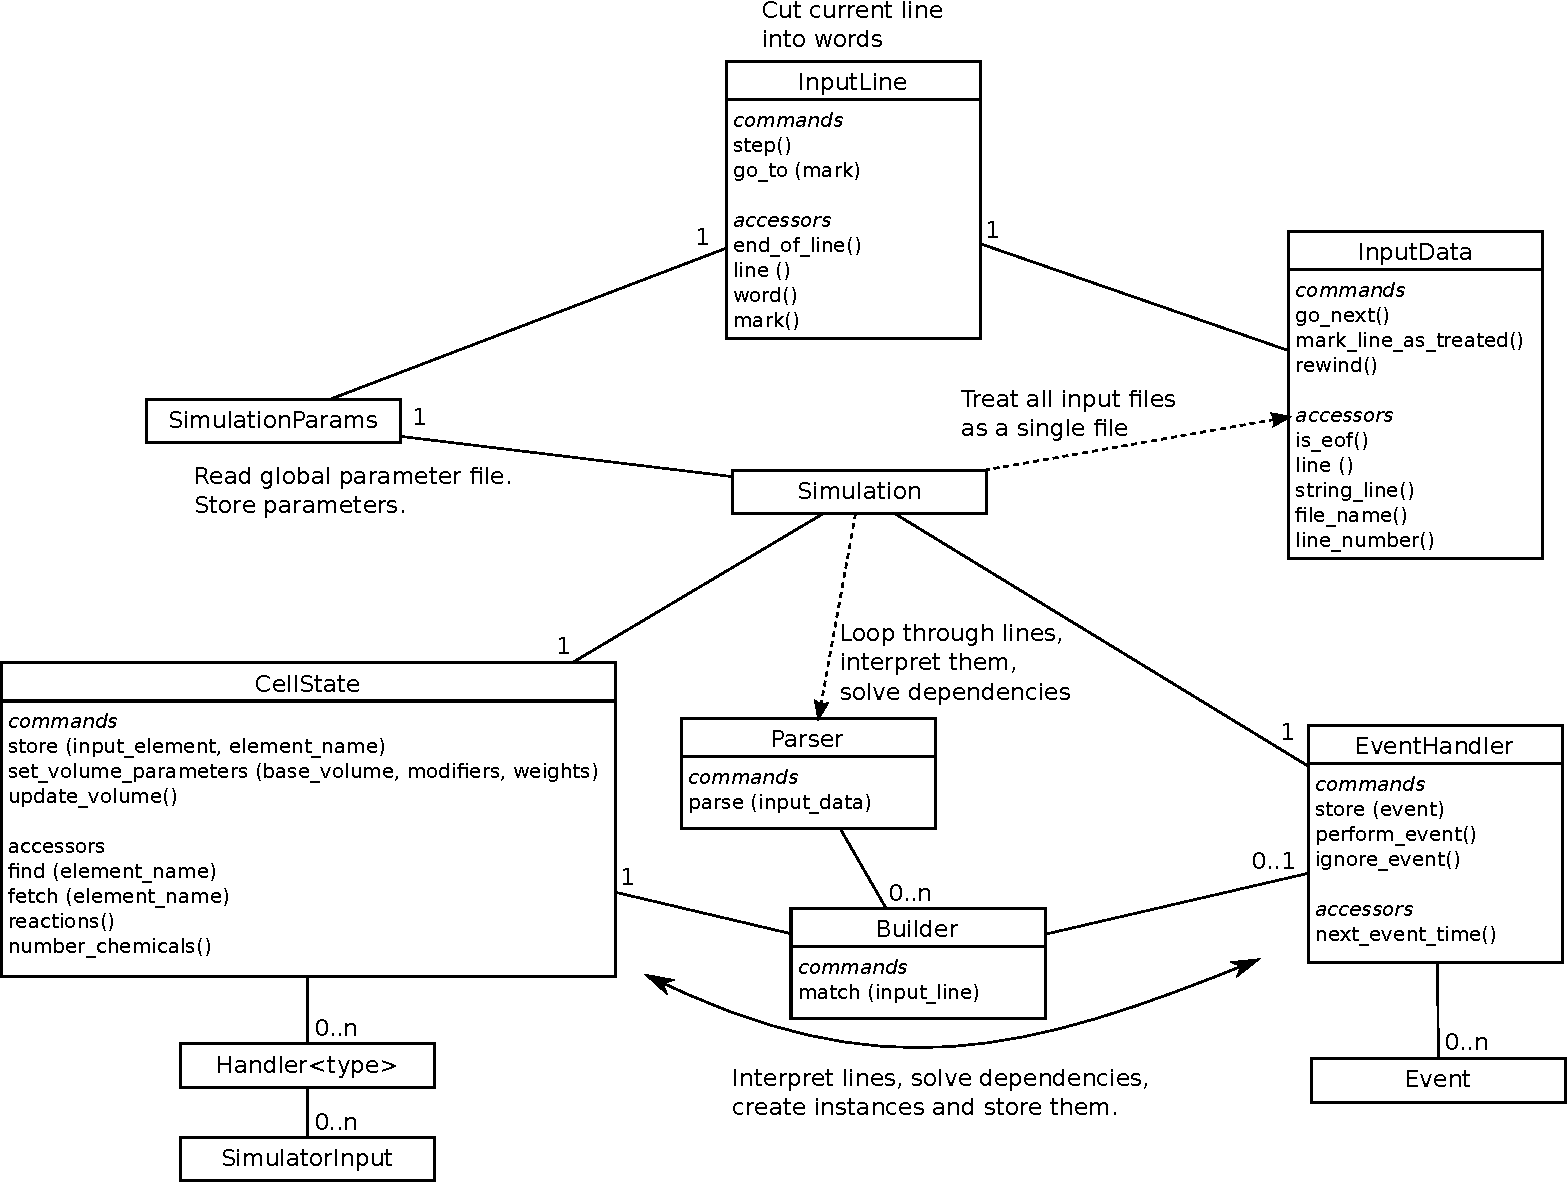
\includegraphics[width=\linewidth]{text_parser}
  \caption{Architecture of the parsing system. \texttt{SimulationParams} reads the global parameter file and stores parameter values. \texttt{InputData} is used to provide a simplified interface to the input files and mark treated lines. A \texttt{Parser} and \texttt{Builders} are used to make sense of individual lines. Everything that is created is stored in \texttt{EventHandler} (for events) and \texttt{CellState} (for the rest). }
  \label{fig:text_parser}
\end{figure}

The parsing system used by the simulator is pretty simple~\reffigp{fig:text_parser}. A \texttt{SimulationParams} class is used to store simulation parameters (which will be used to create and drive the \texttt{Solver}), \texttt{CellState} stores reactions to integrate and \texttt{EventHandler} stores events. At the moment, an \textit{ad hoc} input format is used.

\paragraph{Perspectives} Review \texttt{SimulatorInput} arborescence which seems uselessly complicated. Design an architecture that can handle multiple input formats (plain text or XML).

\subsubsection{Builder and interpreter}

\begin{figure}[!h]
  \centering
  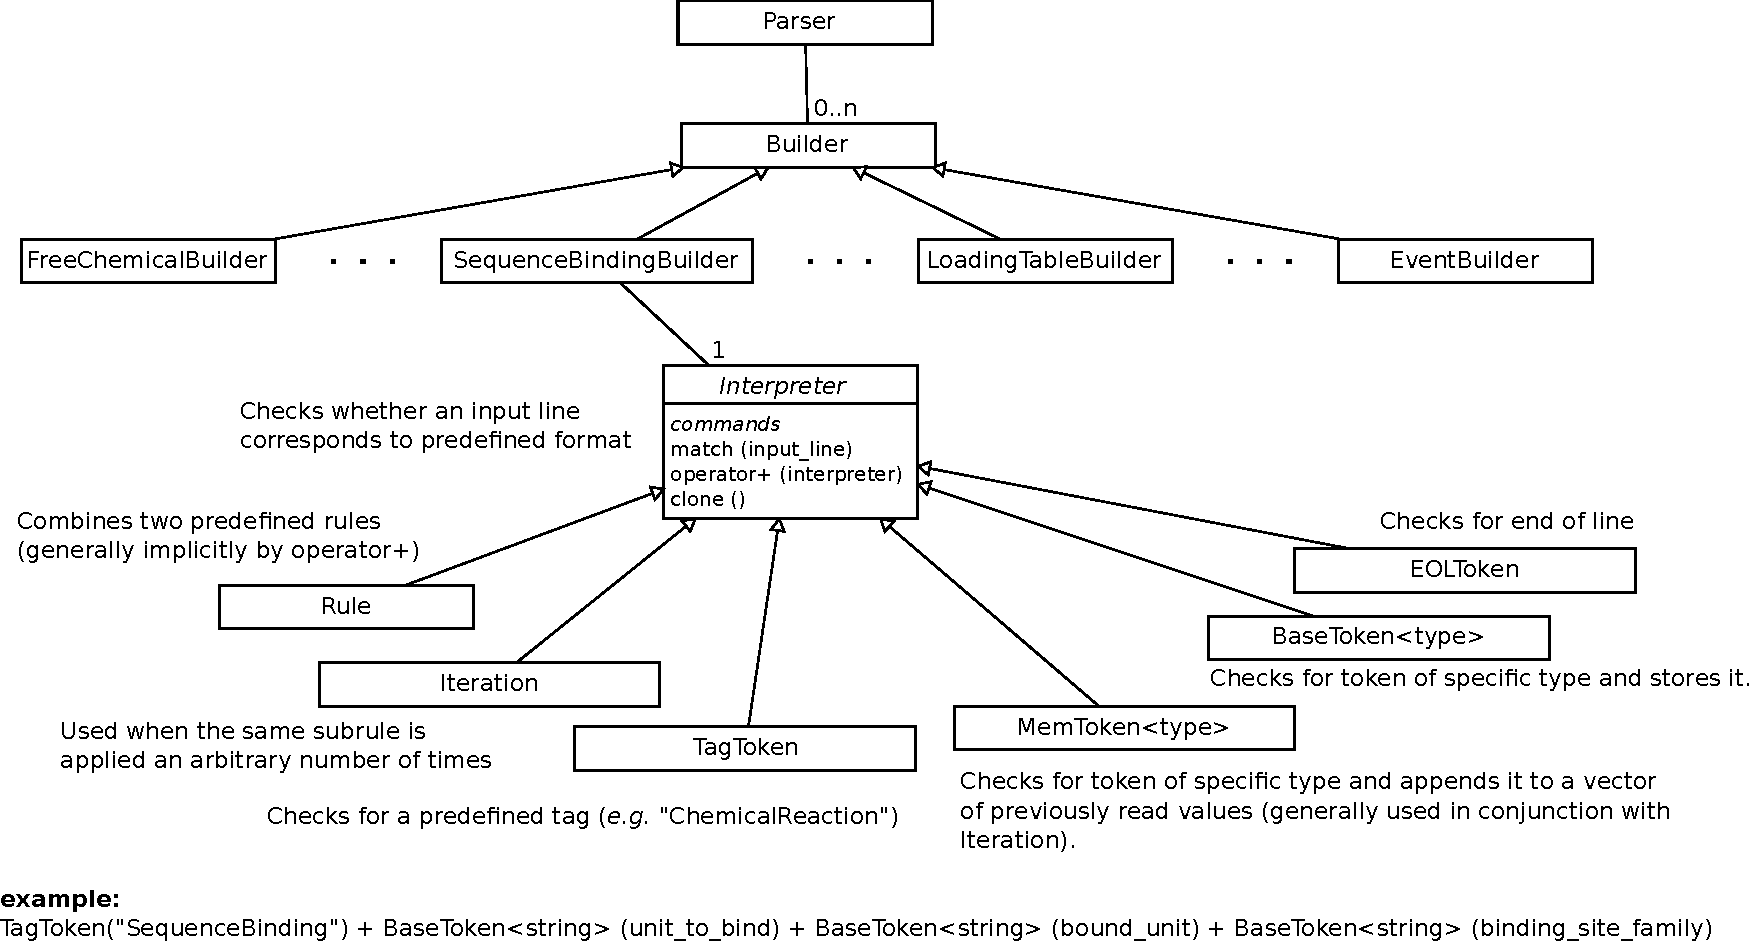
\includegraphics[width=\linewidth]{interpreter}
  \caption{Interpreter system used. For each class of the simulator, a \texttt{Builder} is responsible for interpreting current line, solving dependencies, checking validity of parameters. If format is invalid or dependencies could not be resolved, exceptions are raised to warn the user.}
  \label{fig:interpreter}
\end{figure}

The parsing system is designed to cut each line into words, then the words are interpreted by \texttt{Builder}s that try to create instances of each of the class of the simulator. The \texttt{Parser} loops through the \texttt{Builder}s until an instance was successfully created. Line format is checked token-wise by an \texttt{Interpreter}~\reffigp{fig:interpreter}. If no \texttt{Builder} is able to match the line, a \texttt{FormatException} is raised. If some dependency could not be solved, a \texttt{DependencyException} is raised. In the latter case, the \texttt{Parser} will postpone the line until dependency can be successfully solved.

\paragraph{Perspectives} Maybe create a \texttt{SimulatorToken} to automatically fetch the reference associated to a name? However, this has to be done with care because the right exceptions have to be raised.

\subsubsection{Output}

Two classes are used to produce output. \texttt{ChemicalLogger} logs chemical numbers through time. \texttt{DoubleStrandLogger} logs partial strands of a \texttt{DoubleStrand}.

\paragraph{Perspectives} A \texttt{ReactionLogger} would actually be nice...
